\section{The 2-3 atmospheric sector }

In this subsection we will describe the status of the so called atmospheric neutrino oscillations, i.e. the 2-3 oscillations that were first discovered in the study of atmospheric neutrinos and later were precisely measured with the use of long baseline neutrino beams.   


\subsection{The atmospheric neutrino flux}

The atmosphere is constantly bombarded by primary cosmic rays, composed mainly of protons, with a smaller component, $\simeq$ 5\%, of $\alpha$ particles, and even smaller fraction of heavier nuclei. The interaction of these particles with atomic nuclei in the atmosphere produces hadronic showers composed mainly of pions and kaons. The decay of these mesons according to 
$\pi^+ \rightarrow \mu^+ \nu_\mu$ followed by 
$\mu^+ \rightarrow e^+ \nu_e \bar{\nu}_\mu $,
$K^+ \rightarrow \pi^+ \nu_\mu$ and $K_L \rightarrow \pi^+ e^- \nu_e$
together with their charge conjugated processes produces a flux of $\nu_\mu$ and $\nu_e$ with a steeply falling power-law spectrum (Fig. \ref{fig:nuatmflux}), approximately $E^{-2.7}$ in the region above 1 GeV.   


\begin{figure}[htbp]
\begin{minipage}[c]{.46\linewidth}
%\begin{minipage}[c]
   	      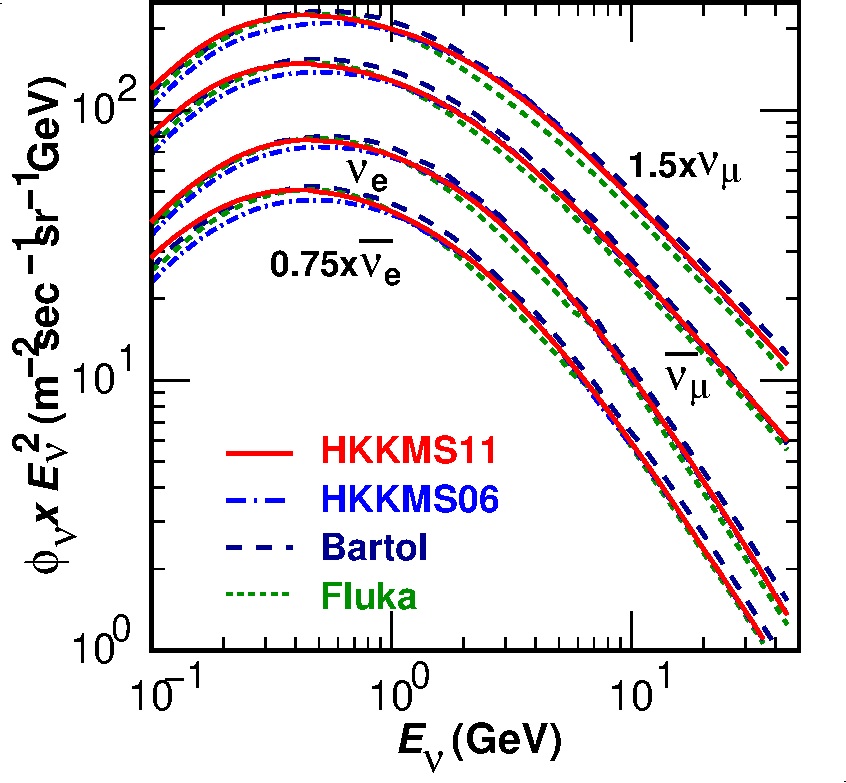
\includegraphics[width=0.9\linewidth]{figures/fig7a-c.pdf}
   \end{minipage} \hfill
   \begin{minipage}{.46\linewidth}
      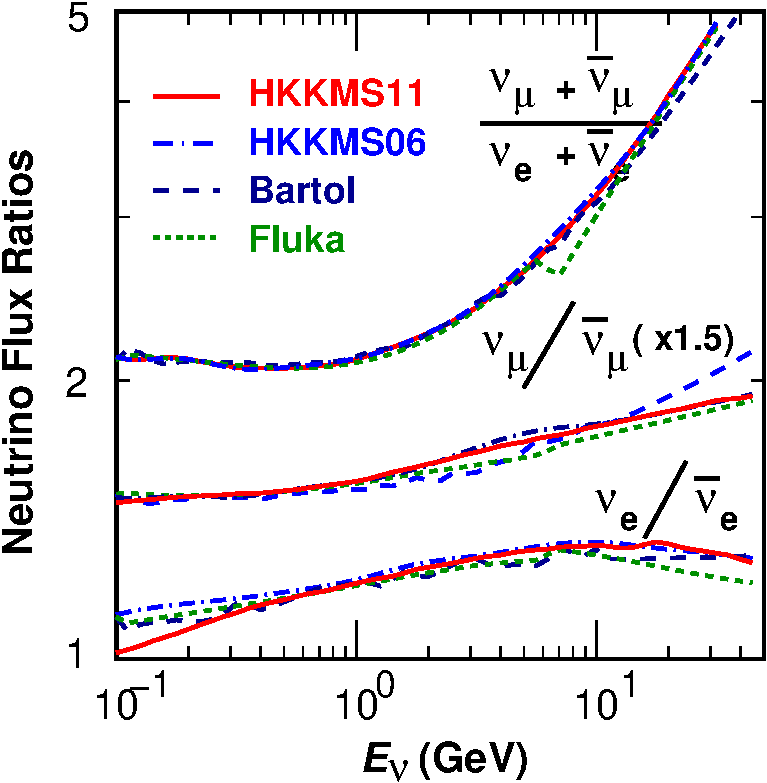
\includegraphics[width=0.9\linewidth]{figures/fig7b-c.pdf}
   \end{minipage}
    \caption{The flux of atmospheric neutrinos (left) and several flux ratios (right) \cite{PhysRevD.83.123001}. }
 \label{fig:nuatmflux}
\end{figure}


The calculation of this neutrino flux \cite{Gaisser:2002jj} relies on the knowledge of the primary flux and composition, of the Earth magnetic field, and of the hadro-production cross-section. Recent studies \cite{PhysRevD.83.123001,Barr:2004br,Battistoni:2002ew} taking into account 3D effects and recent measurements of the hadro-production cross-sections largely improve on previous efforts and reach precisions of 7-8 \% for the flux in the 1-10 GeV range. It should be noticed that the ratio $N(\nu_\mu + \bar{\nu}_\mu)/N(\nu_e + \bar{\nu}_e)$ is predicted with a much better precision of a few \% as several systematic uncertainties cancel in this ratio. In the limiting case where all the muons from pion decays decay themselves in flight, this ratio is close to 2, as can be easily deduced from the decay processes mentioned above.

%\subsection{The early days, the up-down asymmetry and controversy}

\subsection{Interaction of high energy neutrinos with the nucleus}

The interaction of neutrinos with matter takes place through charged current (CC) interactions (exchange of a $W$ boson, production of a charged lepton in the final state) or neutral current (NC) interactions (exchange of a $Z^0$ boson). 
Above a few hundred MeV neutrino energy interactions with the nucleus have a typical $q^2$ which is of the order of one fermi, and the neutrino scatters off individual nucleons inside the nucleus. These interactions (Fig.~\ref{fig:xsec}) can be classified as:
\begin{itemize}
  \item (Quasi-) Elastic interactions, where the finale state nucleon is ejected from the nucleus as a proton or neutron, 
  \item excitation of a nucleon resonance like the $\Delta$,
  \item Deep Inelastic scattering at large energies and for large momentum transfers, where the neutrino interacts with the partons inside the nucleons.
  \end{itemize}  

The Charged Current Quasi elastic process $\nu_l \: n \rightarrow l \: p$ where $l=e,\mu$ plays a special role because it is the dominant process below 1 GeV. Moreover its simple final state is very suitable to the reconstruction of the neutrino energy based on the measurement of the outgoing charged lepton. Neglecting Fermi momentum, the reconstructed neutrino energy is 
\begin{equation}
E_\nu = \frac{m²_p - (m_n-E_b)² - m²_l + 2 (m_n-E_b)E_l}{2 (m_n - E_b - E_l + p_l \cos \theta)}
\end{equation}
 where $E_b$ is the effective binding energy necessary to extract the nucleon from the nucleus, $m_p$ $m_n$ and $m_l$  are the proton, neutron and lepton mass, $E_l$, $p_l$ and $\theta$ are the reconstructed lepton energy, momentum and angle with respect to the beam. This process is particularly suited for Cherenkov detectors, because, while the proton and most of the pions in these interactions are below the detection threshold, electrons and muons can be easily detected, reconstructed and identified. 

In the simplest approach to the calculation of the cross-section, the nucleus is simply parametrized by the Fermi momentum and the binding energy $E_b$. The CCQE cross-section is then mainly governed by the axial vector form factor of the nucleon, where usually a dipole form is assumed
$ G_A (q²) = \frac {g_A} {(1+q²/M²_A)}$.
Most parameters are determined from electron scattering for the vector from factors, and from nuclear $\beta$ decays for $g_A$, leaving the axial mass value $M_A$ as the main free parameter. This simple approach failed, as revealed by the fact that the value of $M_A$ 1.2-1.3 GeV/c$²$ measured by K2K and  MiniBoone for interactions on carbon was very different from the value 1.03 GeV/c$²$ obtained from the analysis of neutrino interactions on deuterium (Fig.~\ref{fig:xsec}).

\begin{figure}[htbp]
\begin{minipage}[c]{.46\linewidth}
%\begin{minipage}[c]
   	      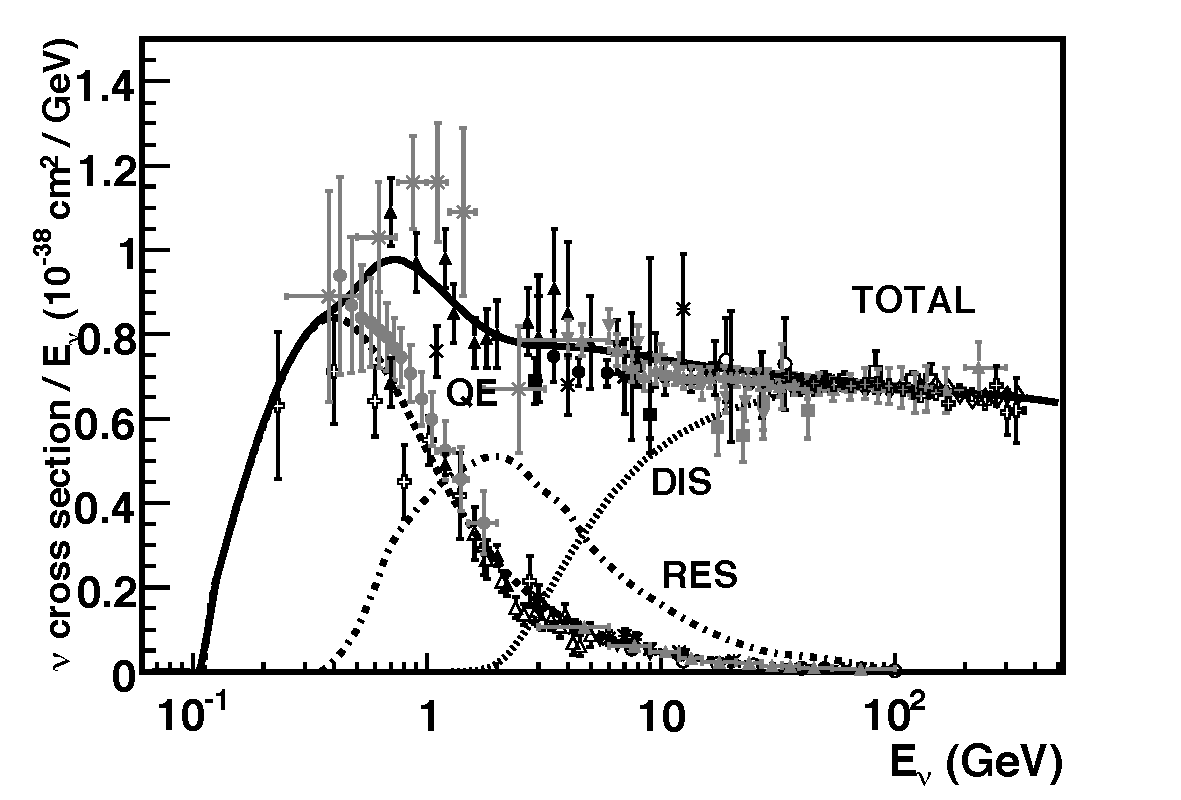
\includegraphics[width=0.9\linewidth]{figures/cc_inclusive_nu.pdf}
   \end{minipage} \hfill
   \begin{minipage}{.46\linewidth}
      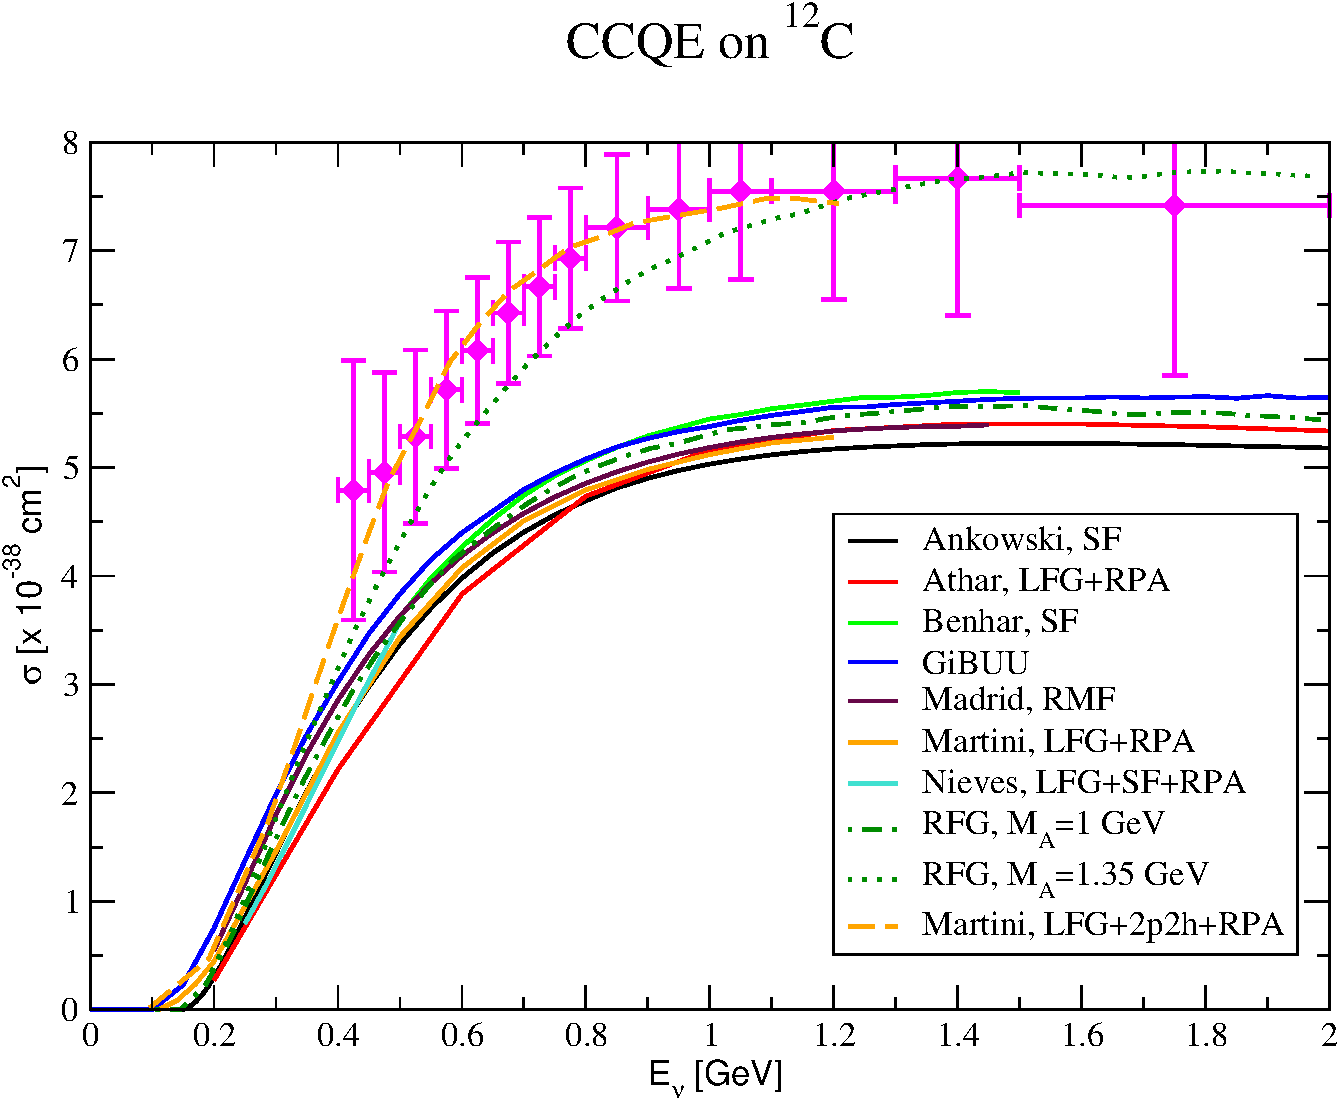
\includegraphics[width=0.9\linewidth]{figures/CCQE_C_2.pdf}
   \end{minipage}
    \caption{ Left plot: Total neutrino per nucleon CC cross sections (for an isoscalar target) divided by neutrino energy and
plotted as a function of energy~\cite{formaggio}.
Right plot: CCQE cross-section on carbon~\cite{alvarez}.
The solid
lines denotes various models.  The dash-dotted and
dotted lines are two models with $m_A=1$ and 1.35 GeV respectively. 
The dashed line takes into account the 2p-2h.  The data points
are from MiniBooNE.}
 \label{fig:xsec}
\end{figure}

A partial solution to this discrepancy came from considering additional processes like interaction of the neutrino with a correlated pair of nucleon inside the nucleus. From the experimental point of view, these processes, named two particle-two hole (2p-2h), cannot be distinguished from CCQE interactions, as low momentum are generally not detected. These processes can represent 10-20 \% of the CCQE cross-section. Despite this progress, the normalization and shape of this additional contribution is still not well-known and model-dependent.

Other nuclear effects, like Final State Interactions (where the ejected nucleon reinteracts within the same nucleus), introduce smearing and corrections which are difficult to evaluate, especially for relatively large nuclei like Carbon, Oxygen, Argon and Iron generally used in these experiments. 
The anti-neutrino cross-sections are even less established with poorer measurements, as it is the case for the $\nu_e$ cross-sections required by the oscillation experiments.  


All these cross-sections are the object of an intense theoretical and phenomenological activity \cite{zeller,martini} given their relevance for oscillation analyses. The knowledge of these cross-sections is still model-dependent and the precision does not exceed the 10-20 \% level. Therefore, most of the experiments include near detectors to study the event rates before oscillations intervene. Clearly a more focused effort, combining phenomenological developments and well controlled experimental data is required for future high precision oscillation experiments.


\subsection{The evidence for atmospheric neutrino disappearance}
\label{subsec:atmevidence}
%from Super-Kamiokande}

The study of atmospheric neutrinos started in the 1960: two experiments in very deep mines, in South Africa \cite{Reines:1965qk} and in India \cite{Achar:1965ova}, observed muons produced by their interactions. 
In the 1980, several massive underground experiments, mainly motivated by the search for the proton decay predicted by Grand Unification theories, started collecting data. These experiments needed to study in detail atmospheric neutrino interactions as they constitute a background for proton decay searches.

In 1988, Kamiokande reported a deficit in the number of $\nu_\mu$ of events, while the number of $\nu_e$ events agreed with the prediction. This initiated the so-called atmospheric neutrino anomaly. This deficit was also observed by the IMB experiment and later by MACRO and SOUDAN-2, while Fr\'ejus and NUSEX observed no deficit. 

The situation evolved rapidly with the advent of Super-Kamiokande~\cite{sknim}, that started data-taking in 1996. Super-Kamiokande is very large water Cherenkov detector located in the Mozumi mine (Gifu prefecture, Japan), under a 1000 m rock overburden, equivalent to 2700 m of water. It is a stainless steel tank (41.4 m high, 39.3 m diameter) containing 50 kt of ultra-pure water. The detection volume is partitioned in an outer detector, composed of 1885 8 inch PMTs, and an inner detector with 11146 20 inches PMTs. The fiducial volume is 22.5 kt. Super-Kamiokande could rapidly accumulate a rather large data set of atmospheric neutrinos, measuring the direction of the produced lepton, its energy for fully contained events and their nature. Above a few hundred MeV/c, the direction of the produced lepton is strongly correlated to the direction of the incoming neutrino.

Super-Kamiokande classifies events as Fully Contained (where the neutrino interaction takes place inside the inner detector and all the particle stop in the same volume), Partially Contained (some particles escape to the outer detector) and Upward Going muons, where the neutrino interacts in the rock below the detector. The events can be further classified according to the number of Cherenkov rings observed, the observed total energy, the number of decay electrons. Electrons and muons can be reliably identified (the misidentification probability is 0.7 \%) on the basis of the ring properties. Cherenkov rings produced by muons have sharp edges while in the case of electrons the photons are produced by the numerous electrons and positrons in the electromagnetic shower, with angular dispersion due to scattering, resulting in a ring with diffuse edges. The momentum resolution for isolated ring produced by a lepton of momentum $p$ is $0.6\% +2.6\%/\sqrt{p ({\rm GeV/c})}$. Sub-threshold muons and charged pions can be tagged by the presence of a delayed electron from muon decay.

In 1998, the Super-Kamiokande collaboration presented their first analysis of atmospheric neutrinos~\cite{Fukuda:1998mi}, in particular the distributions of zenith angle for $ \nu_\mu$ and $\nu_e$ event selections (see Fig.~\ref{fig:sk-atm} for an updated distribution) based on an exposure of 33 kton year. This was the first compelling evidence for neutrino oscillations as the explanation of the previously mentioned anomaly.  

Indeed the neutrino path from the production to the detection varies from 15 km for down-going neutrinos (cosine of the zenith angle equal to 1) to more than 12000 km for up-going neutrinos having traversed the whole Earth (cosine of the zenith angle equal to -1), thereby probing a large span of possible oscillation lengths. 

In a two neutrino scenario, the $\nu_\mu$ disappearance is governed by 
\begin{equation}
\sin^2 (2 \theta) \sin^2 (4 \Delta m^2 L /E),
\end{equation}
where $\theta$ is the relevant mixing angle and $\Delta m^2$ the squared-mass difference of the mass eigenstates. A glance at Fig.\ref{fig:sk-atm} reveals several important overall features: 
\begin{itemize}
\item there is a strong disappearance of $\nu_\mu$, especially visible for up-going neutrinos. As the survival probability for very long baseline approaches $1/2 \sin^2 (2 \theta)$, and the observed survival probability is close to 0.5, the mixing angle is therefore close to the maximal value $\pi/4$. 
\item The disappearance sets in for neutrinos close to horizontal zenith angle, and therefore the oscillation length should be of the order of 400 km for energy around 1 GeV, or $\Delta m^2 \simeq 10^{-3}$eV$^2$.  
\item There is no sizeable excess or deficit of $\nu_e$. Therefore the oscillations of $\nu_{\mu}$ should mainly involve either $\nu_{\mu} \rightarrow \nu_{\tau}$ or $\nu_{\mu} \rightarrow \nu_s$, where $\nu_s$ is an additional neutrino state.
\end{itemize}


\begin{figure}[htbp]
\centering
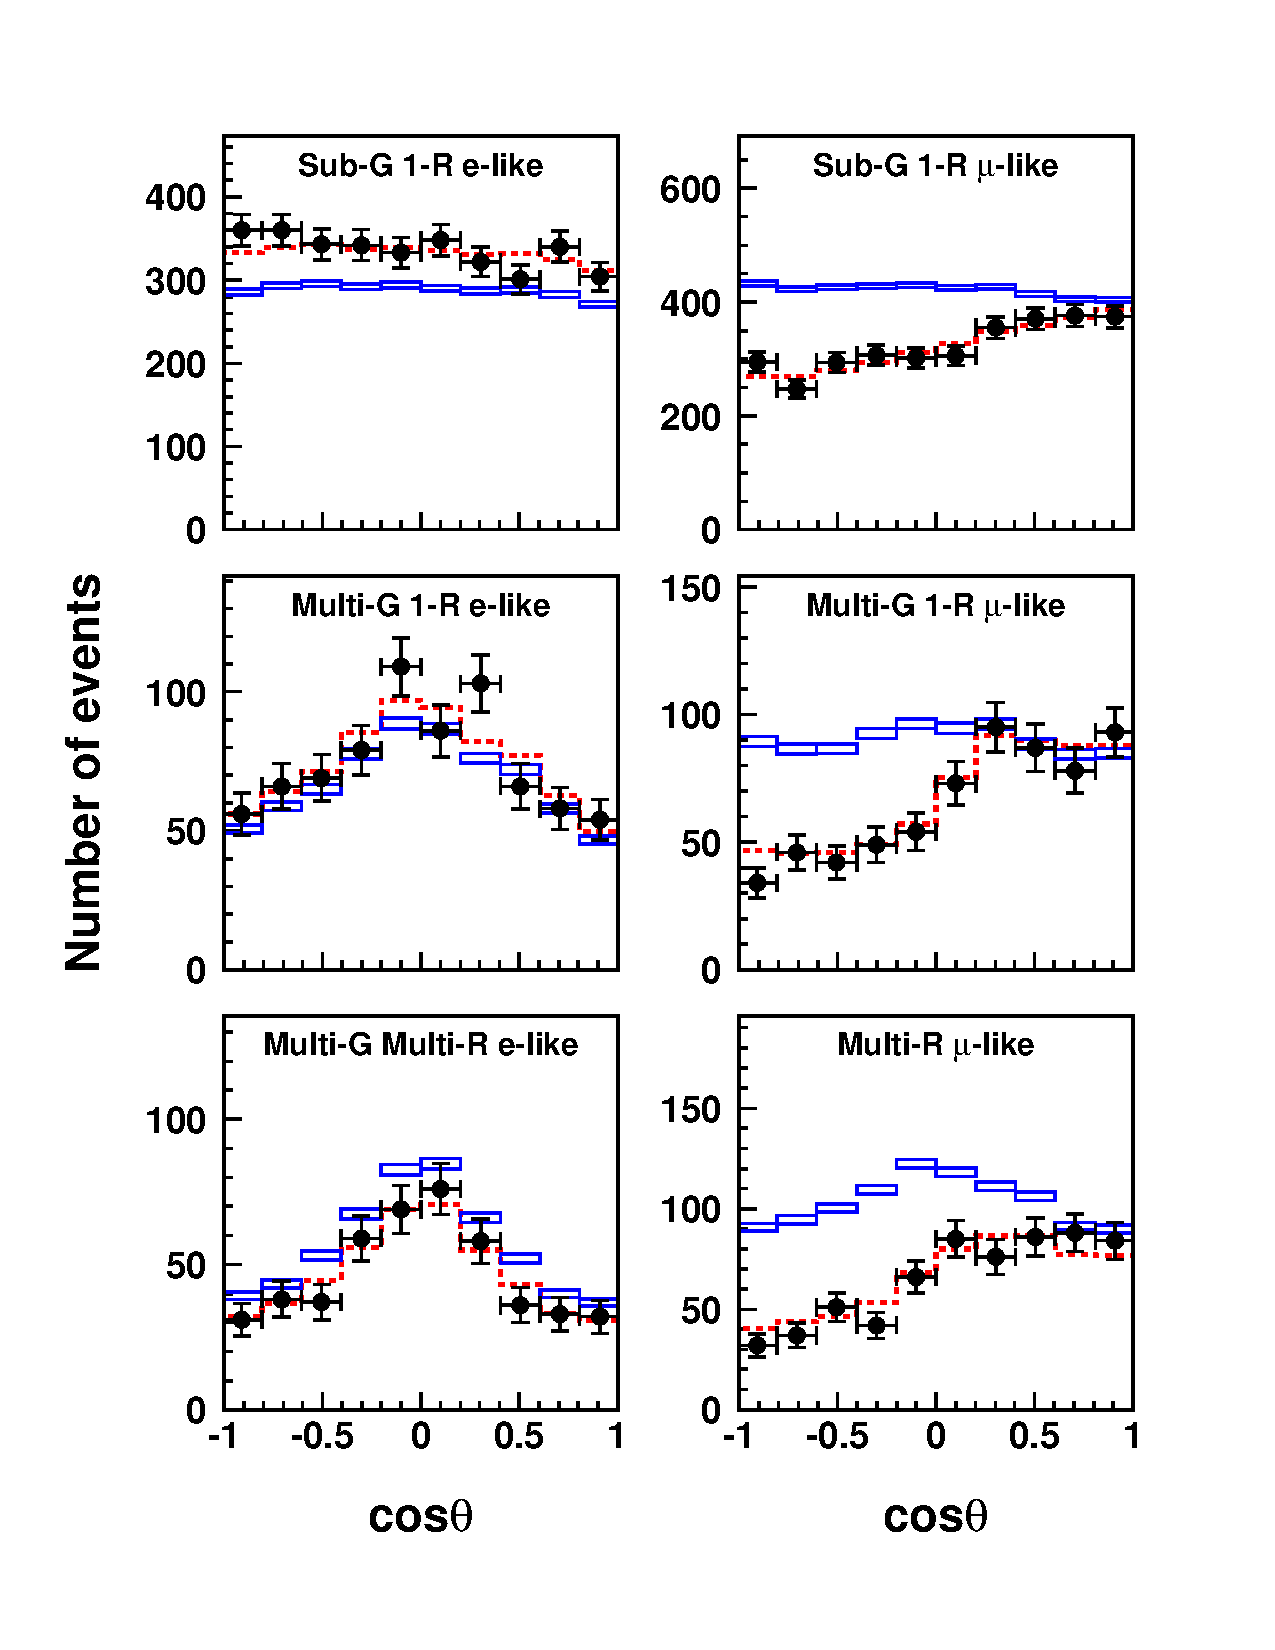
\includegraphics[width=0.8\linewidth]{figures/sk-2006-atm.pdf}
  \caption{Zenith angle distributions of Super-Kamiokande atmospheric neutrino events from \cite{Hosaka:2006zd}. Fully contained
e-like, $\mu$-like events
are shown for data (filled circles with statistical
error bars), MC distributions without oscillation (boxes)
and
best-fit distributions (dashed). The box height shows the
statistical error.}
 \label{fig:sk-atm}
 \end{figure}

Independently of any accurate predictions of the neutrino flux, the experimental observation of the distributions of Fig.\ref{fig:sk-atm} is sufficient to make a strong case for neutrino disappearance. Indeed, above several GeV, the neutrino flux is isotropic, as the primary cosmic rays are not deflected in a significant way by the geomagnetic field. The observation of a zenith angle dependent deficit of the neutrinos is then a sufficient argument to conclude that these neutrinos undergo a non-standard propagation.  

While in 1998 other hypotheses like decay or decoherence were still open, more recent data from long baseline accelerator experiments have ruled out all explanations apart from oscillations because the alternative hypotheses imply a different L/E behaviour. 
    
The IceCube experiment at the South Pole has recently completed the installation of DeepCore, a denser array of optical modules, aimed at significantly lowering the muon threshold. With data recorded between 2011 and 2014, corresponding to 5074 observed events, they have recently published an analysis of the disappearance of atmospheric $\nu_\mu$  \cite{Aartsen2016161} in the range 10-100 GeV, requiring the zenithal angle to satisfy $\cos \theta < 0$,  which has a similar sensitivity to that of Super-Kamiokande (Fig. \ref{fig:icecubeosc}) with the prospects of further improvements. 


\begin{figure}[htbp]
\centering
%\includegraphics[width=0.5\linewidth]{energy_miniboone.eps}
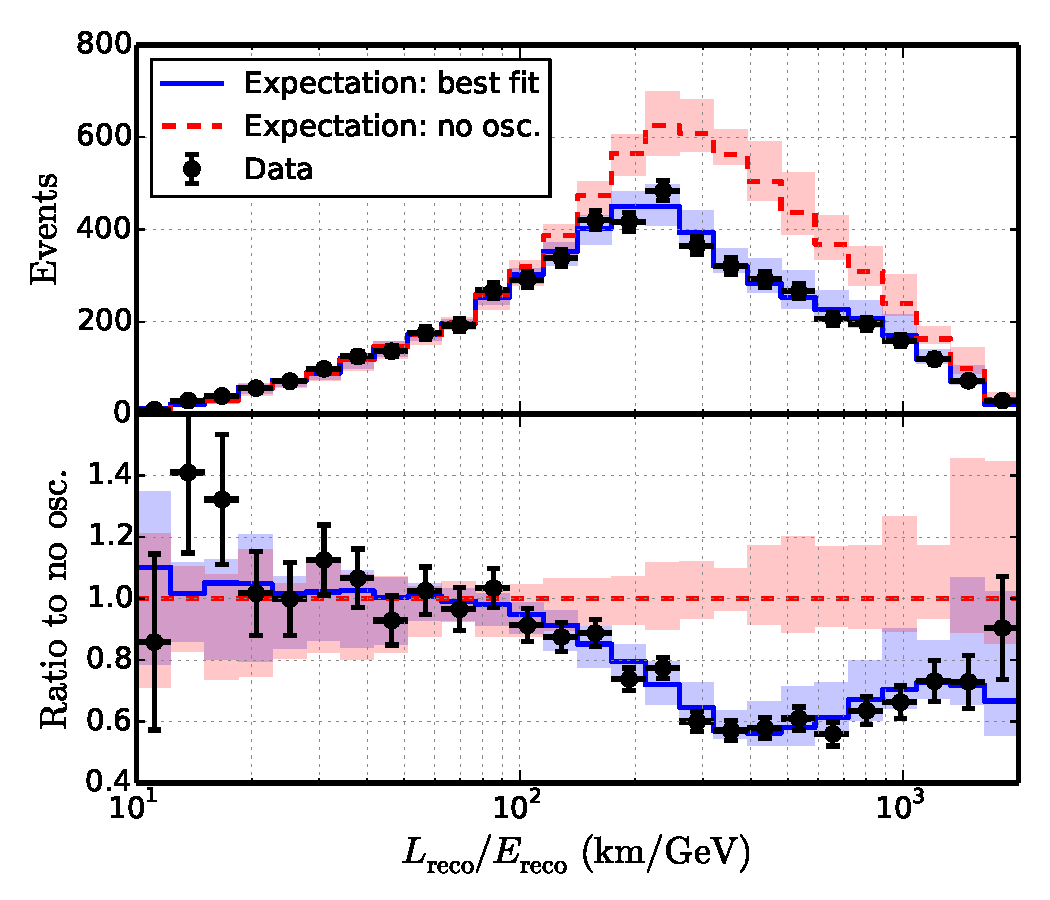
\includegraphics[width=0.6\linewidth]{figures/icecube_osc2014_data_mc_LE.pdf}
  \caption{Distribution of atmospheric neutrino events measured by the IceCube experiment\cite{Aartsen2016161} as a function of
reconstructed L/E. Data are compared to the best fit and
expectation with no oscillations (top), and the ratio of data
and best fit to the expectation without oscillations is also shown
(bottom). Bands indicate estimated systematic uncertainties.}
 \label{fig:icecubeosc}
 \end{figure}